\documentclass{article}
% Allow the usage of utf8 characters
\usepackage[utf8]{inputenc}
\usepackage{listings}
\usepackage{graphicx}



% Start the document
\begin{document}

\section*{1}
The total tree diagram is as followed.\\
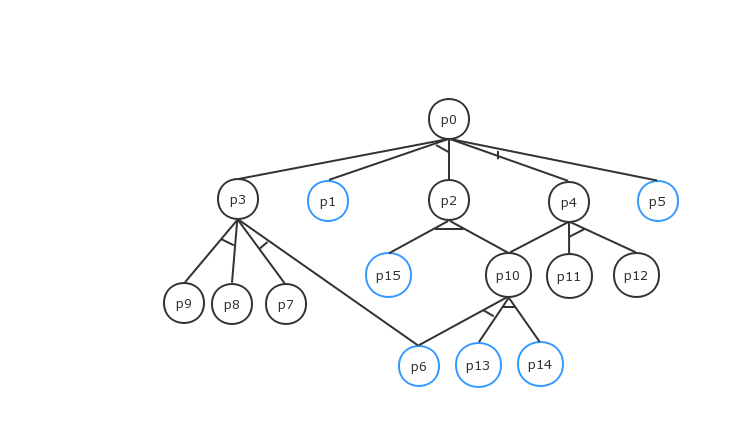
\includegraphics[scale=0.45]{result1.jpg}\\

And for this tree, the output is as followed.\\
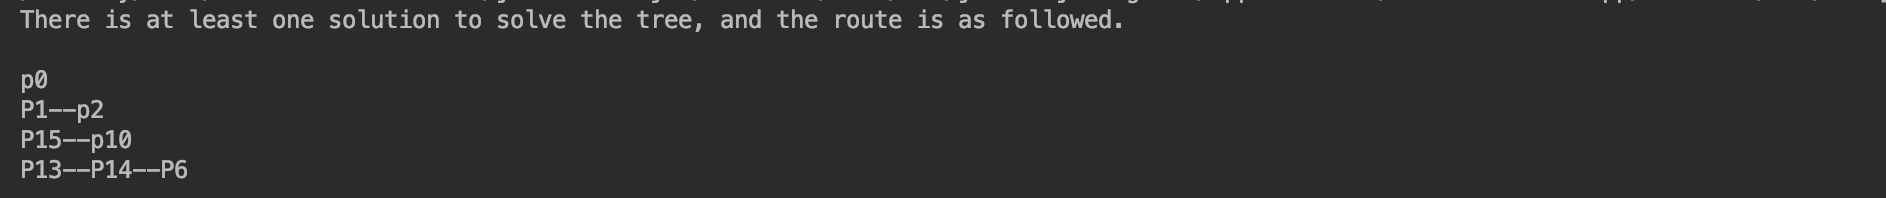
\includegraphics[scale=0.365]{output1-1.png}\\
\newpage
\section*{2}

The total tree diagram is as followed.\\\\
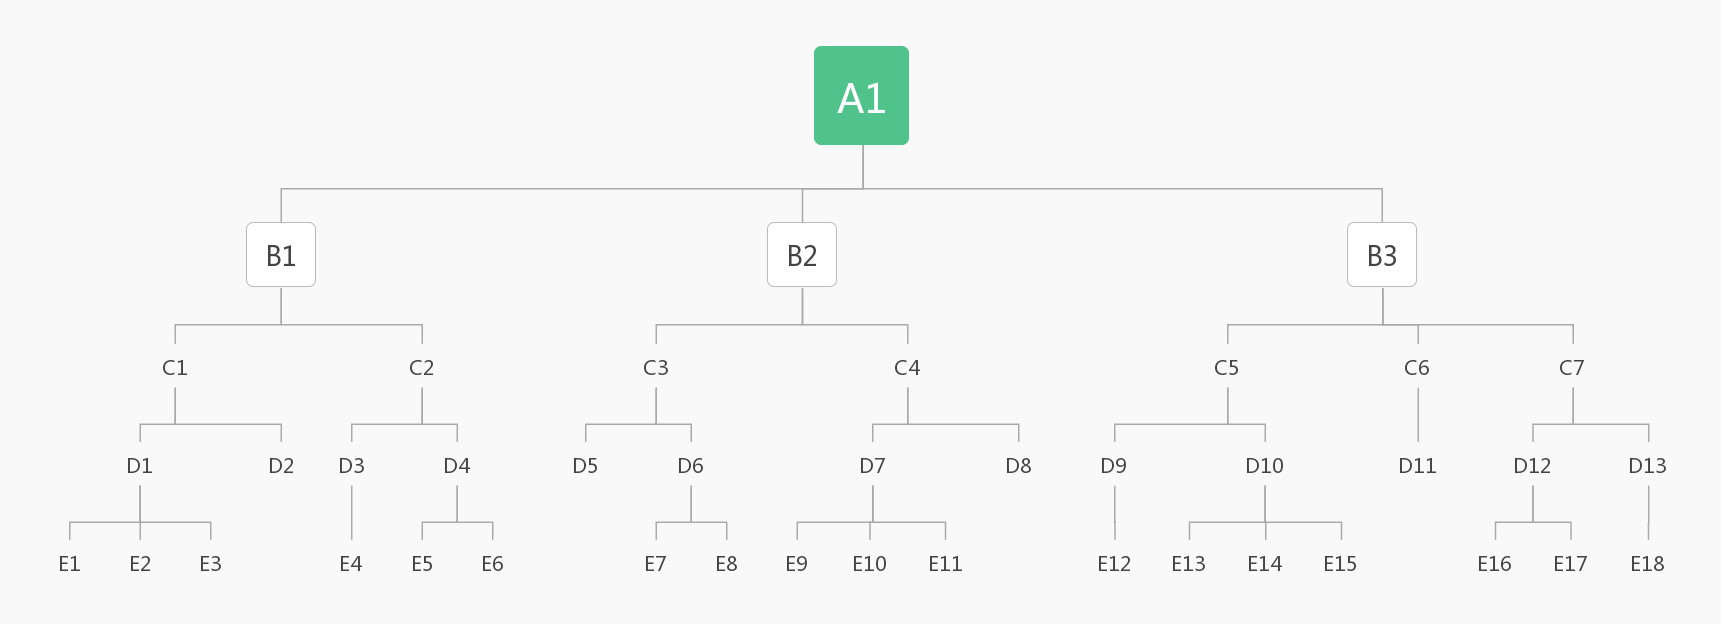
\includegraphics[scale=0.2]{result2.jpg}\\

For the values of d-level and e-level are randomly generated between 0-99, so the results may differ each time.\\

Here are two example result : \\\\
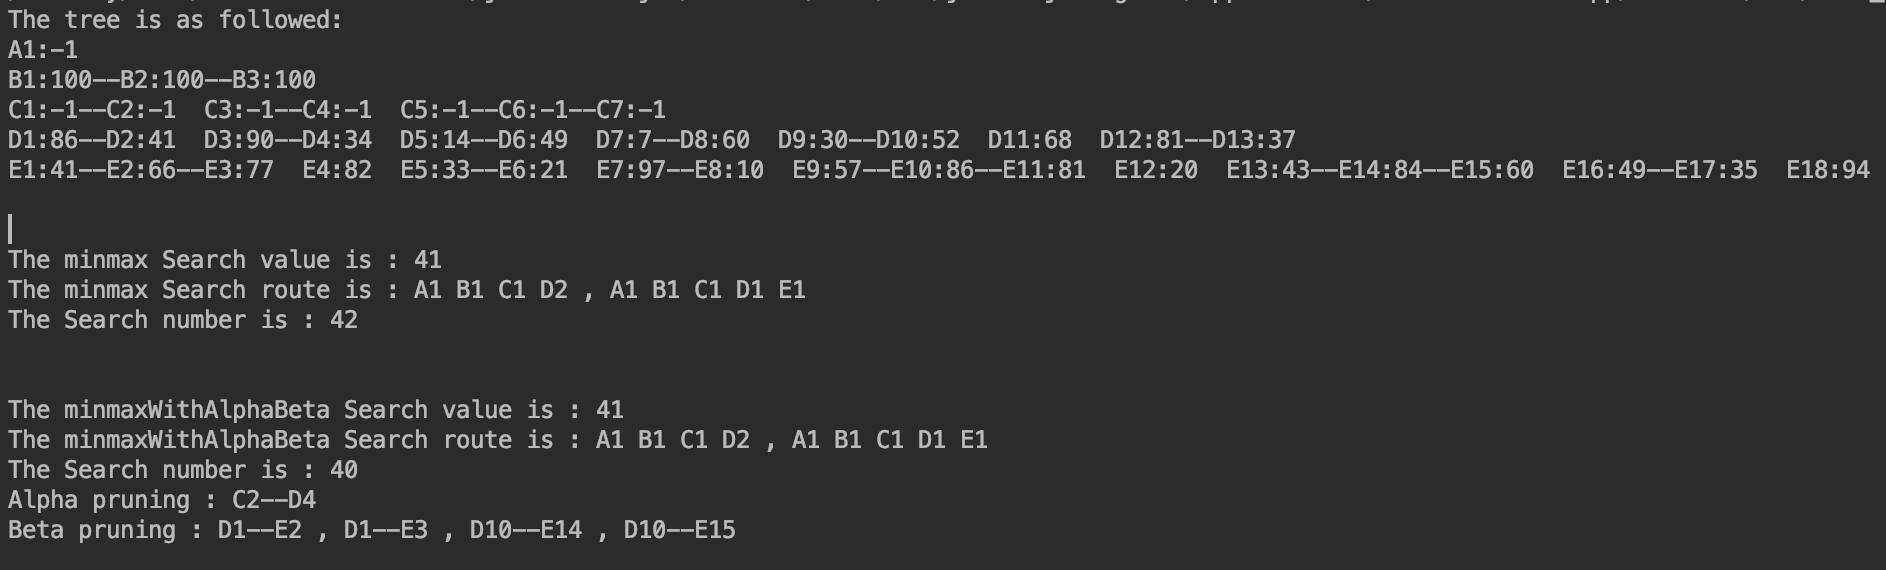
\includegraphics[scale=0.365]{output2-1.png}\\
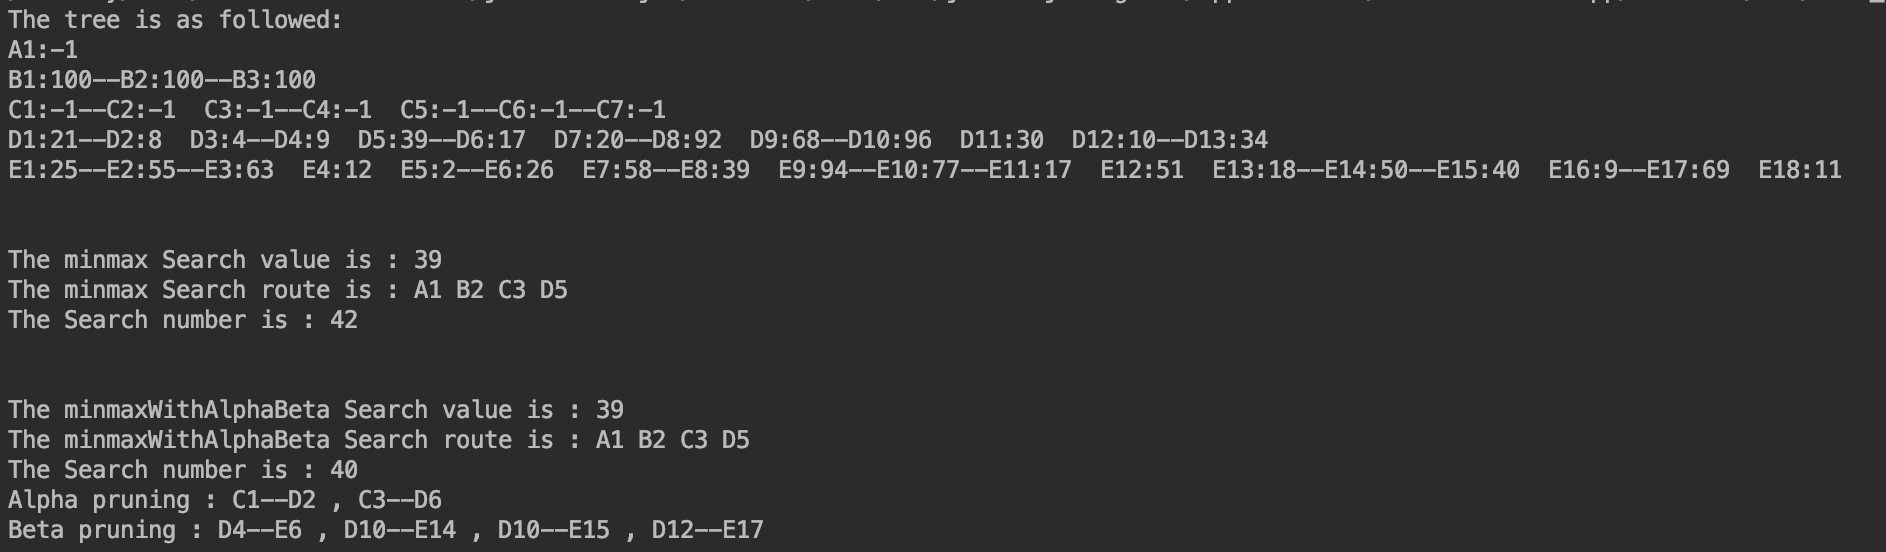
\includegraphics[scale=0.365]{output2-2.png}\\\\

In the ordinary tree, c-level and above are nodes without solutions. For the odd levels being maximum levels, so the values are -1 means minus infinite. 100 means infinite.\\

In the result we can see that it cost less search times in Alpha-Beta Pruning which means that it is more efficient.\\

Also there are still some problems in the experiment. There are no leaf nodes without any solution values. But it doesn't influnce the result.

\newpage


\end{document}